\begin{figure}[ht]
\centering
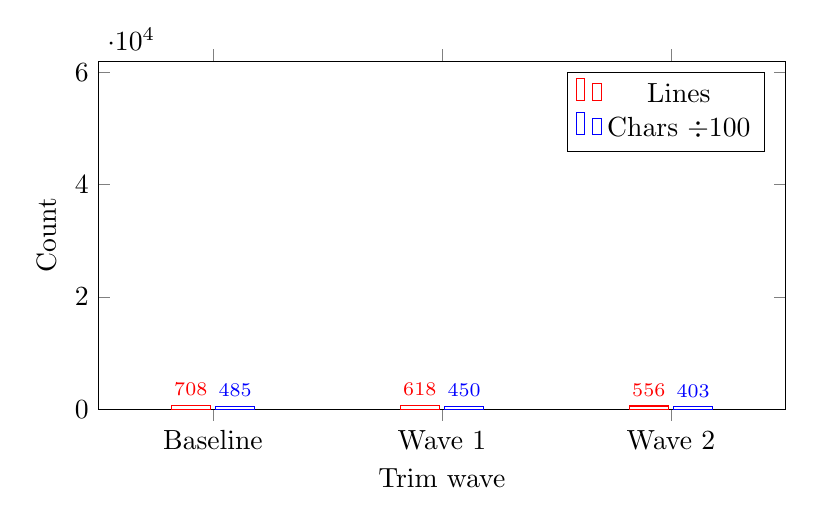
\begin{tikzpicture}
\begin{axis}[
  ybar,
  bar width=14pt,
  width=0.85\textwidth,
  height=6cm,
  enlarge x limits=0.25,
  symbolic x coords={Baseline, {Wave 1}, {Wave 2}},
  xtick=data,
  xlabel={Trim wave},
  ylabel={Count},
  ymin=0,
  ymax=62000,
  legend style={at={(0.97,0.97)}, anchor=north east},
  nodes near coords,
  nodes near coords align={vertical},
  every node near coord/.append style={font=\scriptsize},
  cycle list name=color list,
]
%% Lines series
\addplot coordinates {(Baseline,708) ({Wave 1},618) ({Wave 2},556)};
\addlegendentry{Lines}
%% Chars series (divided by 100 for visual scale, annotated raw)
\addplot coordinates {(Baseline,485) ({Wave 1},450) ({Wave 2},403)};
\addlegendentry{Chars $\div 100$}
\end{axis}
\end{tikzpicture}
\caption{\claudemd size trajectory across Wave~1 (redundancy removal) and
Wave~2 (worktree-isolation externalisation); 21.5\,\% line reduction,
16.9\,\% char reduction.
Char values plotted scaled by $1/100$; raw values:
Baseline~48\,487, Wave~1~44\,974, Wave~2~40\,309.
Source: \texttt{data/aggregated/trim-results.csv}.}
\label{fig:size-trajectory}
\end{figure}
